% !TEX root = ../ICRA19Hybrid.tex

\section{EXPERIMENTS} % (fold)
\label{sec:experiments}
\begin{figure}[h]
    \centering
    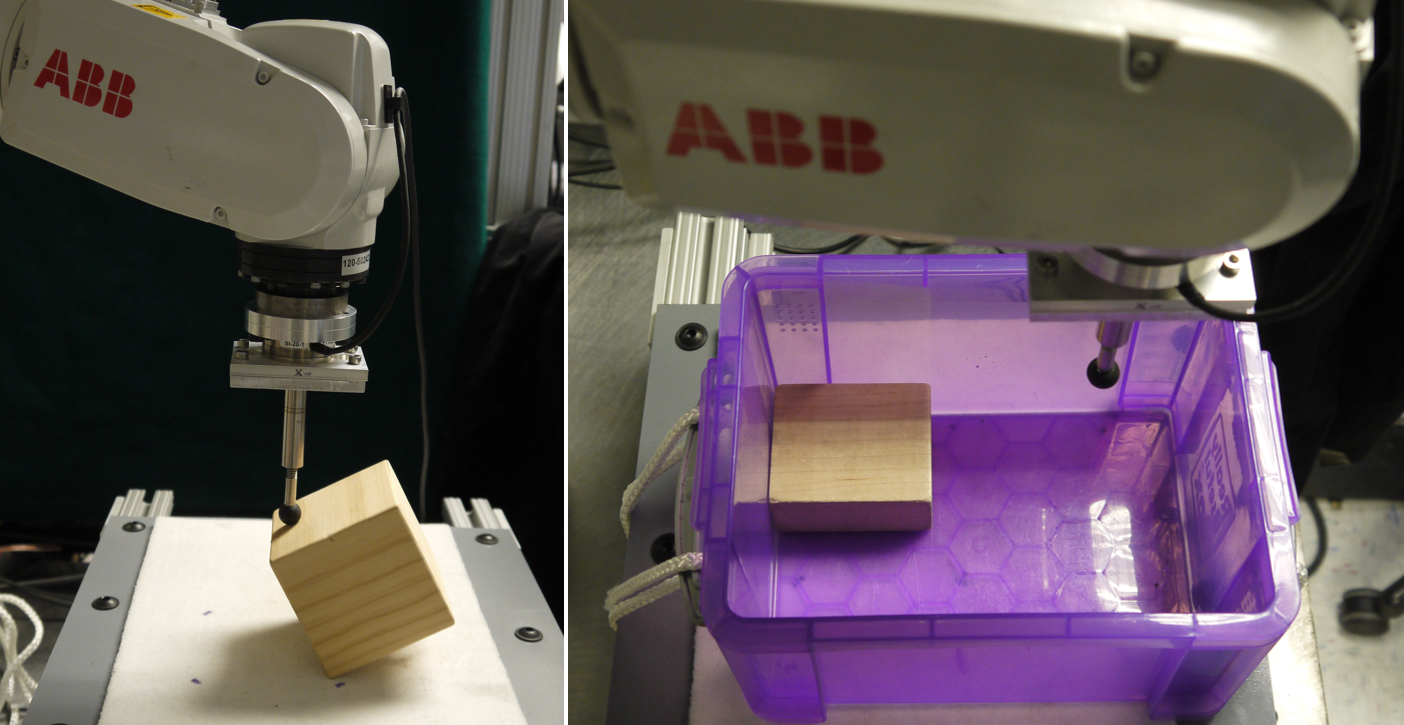
\includegraphics[width=0.5\textwidth]{figs/experiment_photo_1.PNG}
    \caption{Our experiment setup. Left: block tilting. Right: tile levering-up.}
    \label{fig:experiment_photo_1}
\end{figure}
We implemented two example tasks: block tilting (section~\ref{sec:example}) and tile levering-up. In the tile levering-up example, the robot need to pivot the object up against a corner in a box. The object is modeled as a cuboid. During the motion, the contacts between the object and the corner are sliding, while the contact between the object and the robot is sticking.

In the block tilting task, the object is a wooden block with edge length 75mm. We place a 2mm-thick piece of cloth on the table to introduce some passive compliance as well as increasing friction. In the tile levering-up example, the object is placed at a corner of a plastic box, which is fixed in space. We experimented with a variety of objects.
The robot hand is a metal bar with a rubber ball installed on the tip to increase friction.

We implemented our algorithm \ref{alg:solve_for_velocity} and \ref{alg:solve_for_force} in both Matlab and C++. The projected gradient descent is the most time-consuming part of our algorithm. With $N_s = 3$ initial guesses, the C++ code can solve the block tilting problem in 35ms, solve the levering-up problem in 25ms. The Matlab version is on average 10x slower.

The control computed by our algorithm can be implemented in many ways. We implemented hybrid force-velocity control with position-control inner loop according to \cite{maples1986experiments}, and added functionality for choosing axes in any orientation. We used an ABB IRB 120 robot arm with 250Hz communication (but with 25ms latency), and a wrist-mounted force torque sensor, ATI Mini-40, to measure contact forces at 1000Hz.

We ran the block tilting task 50 times in a row\footnote{You can find the 25min video at \href{https://youtu.be/YIP8xIFATHE}{https://youtu.be/YIP8xIFATHE}}. Each run contains 15 time steps. The robot successfully tilted the block 47 times. The three failures were all stopped prematurely because the robot detected large force (about 25N on the FT sensor) at a time step. The reason could be a bad solution from our algorithm, or the instability of our force control implementation.

We ran the tile levering-up task for about 20 times on different objects. The successful rate is about two-thirds. The failures are caused by unexpected sticking between the object and the wall, or unexpected slipping between the robot hand and the object. One important reason for these failures is the slow response of the low level force control: the commanded positive contact normal force were tracked with large errors, which could surely be improved with better engineering. We did observe that the failures are less likely to happen if the robot moved slower.

\subsection{Resources} % (fold)
\label{sub:code}
The Matlab implementation of the two algorithms along with several examples can be obtained from \href{https://github.com/yifan-hou/pub-icra19-hybrid-control}{https://github.com/yifan-hou/pub-icra19-hybrid-control}.
 % You can also download our implementation of the low level hybrid force-velocity controller from \href{https://github.com/yifan-hou/forcecontrol}{another GitHub repository}.


